\chapter{DynSGX}
\label{chapter:dynsgx}

\section{Introdução}
\label{sec:dynsgx_intro}

Considerando as limitações do SGX apresentadas na Seção~\ref{sec:sgx_limitacoes}
% e as observações feitas nas Seções~\ref{sec:abordagem_particionamento_aplicacoes}
e as observações feitas na Seção~\ref{sec:abordagem_gerencia_memoria}, foi desenvolvida uma ferramenta chamada
DynSGX~\cite{DynSGXCloudCom2017}. DynSGX tem como objetivos: ($i$) permitir o
carregamento e remoção de código dinamicamente em enclaves SGX, ($ii$) garantir
a segurança e privacidade de código, ($iii$) permitir uma melhor gerência de
memória por parte do desenvolvedor e usuário de aplicações SGX, e ($iv$)
facilitar o uso de Intel SGX por desenvolvedores sem conhecimento sobre
programação de aplicações SGX.

DynSGX permite que aplicações seguras sejam inicializadas com enclaves pequenos,
e carregar e remover funções no enclave em tempo de execução, à medida que elas
são necessárias. Isso permite que desenvolvedores e usuários possam gerenciar de
forma melhor o consumo de memória. Além disso, DynSGX faz uso do processo de
atestação remota para estabelecer um canal de comunicação confiável para ser
usado no carregamento e remoção de funções do seu enclave, possibilitando a
privacidade do código das funções.

\section{Componentes}
\label{sec:dynsgx_componentes}

O DynSGX é construído baseado em apenas dois componentes: ($i$) o \texttt{DynSGX
enclave} e ($ii$) o \texttt{DynSGX Client}. O \texttt{DynSGX enclave} funciona
como um TEE, responsável pela segurança e privacidade de código e dados de
desenvolvedores e usuários. O \texttt{DynSGX Client}, por sua vez, funciona como
uma interface entre o \texttt{DynSGX enclave} e seus desenvolvedore de
aplicações e usuários. Outra função do \texttt{DynSGX Client} é automatizar o
processo de conversão de uma aplicação qualquer para uma aplicação segura.
O funcionamento de ambos os componentes é melhor definido nas seções que seguem.

\section{TCB do DynSGX}
\label{sec:dynsgx_tcb}

No \texttt{DynSGX enclave} o TCB é limitado ao Intel SGX SDK e PSW, como
qualquer aplicação SGX, acrescentando-se apenas um conjunto de seis funções
compatíveis com SGX, resultando em um enclave com tamanho inicial de apenas
$1.4\ MB$. Tais funções são usadas para ($i$) realizar o processo de atestação
remota, ($ii$) carregar funções no enclave, ($iii$) executar funções carregadas
dinamicamente, e ($iv$) remover funções do enclave.

Para o processo de atestação remota, apenas a função \textit{enclave\_ra\_init}
precisa ser inserida no enclave. Esta função internamente executa a função
\textit{sgx\_ra\_init} do SDK, que inicia o processo de atestação. Para
carregar funções no enclave, duas funções são necessárias: \textit
{enclave\_get\_fas}, responsável por prover uma lista de funções que já estão
disponíveis no enclave, e \textit{enclave\_register\_function}, responsável por
carregar novas funções no enclave. A função \textit{enclave\_execute\_function}
é utilizada para executar funções carregadas no enclave. Por fim, as funções
\textit{enclave\_unregister\_function} e \textit{enclave\_clear\_functions}
podem ser utilizadas para remover funções do enclave.

O \texttt{DynSGX Client} não é considerado como parte do TCB do DynSGX. Isso
porque ele é um \textit{script} escrito em Python, contendo apenas cerca de $300$
linhas de código, que é executado no ambiente do próprio usuário, podendo ser
facilmente auditado pelo mesmo.

\section{Modelo de programação}
\label{sec:dynsgx_modelo_programacao}

Assim como várias outras ferramentas baseadas em programação na nuvem, DynSGX
segue o modelo cliente-servidor, onde o enclave do DynSGX executa no lado do
servidor, e os desenvolvedores e usuários interagem com ele a partir do lado do
cliente.

DynSGX não requer que desenvolvedores tenham conhecimento sobre como desenvolver
aplicações SGX. Ao invés disso, desenvolvedores podem escrever suas funções como
se estivessem desenvolvendo um programa qualquer na linguagem de programação C.
Após escrever suas funções, uma das ferramentas providas pelo DynSGX, \texttt
{bytes\_extractor} compila o arquivo \textit{.c} que contém o código das
funções, e posteriormente recupera os \textit{bytes} que compõem essas funções.
Os \textit{bytes} recuperados pela ferramenta são então enviados de forma segura
para o enclave do DynSGX, onde são armazenados para uma posterior execução. É
importante mencionar que os arquivos \textit{.c} são compilados com a opção
-fPIC, de modo a gerar um código binário independente de posição.

Para exemplificar esse processo, vamos supor que um usuário deseje computar de
forma segura e privada a soma de dois números inteiros. Para isso, o
desenvolvedor da aplicação escreve uma função chamada \textit{sum\_function},
como a descrita no Código Fonte~\ref{lst:sumFunctionC}.

% \noindent\begin{minipage}{.24\textwidth}
\begin{lstlisting}[language=C, label=lst:sumFunctionC, caption={Exemplo de função C para somar dois números inteiros.}]
int sum_function(int a, int b) {
    return a + b;
}
\end{lstlisting}

Após compilar o arquivo \textit{.c} que contém essa função, a ferramenta \texttt
{bytes\_extractor} recupera os \textit{bytes} do código \textit{Assembler} em
arquitetura \textit{x86-64}, como o exibido no Código Fonte~\ref
{lst:sumFunctionASM}, resultando na seguinte \textit{hexstring}:
{\ttfamily \textbackslash x55\textbackslash x48\textbackslash x89\textbackslash
xe5\textbackslash x89\textbackslash x7d\textbackslash xfc\textbackslash
x89\textbackslash x75\textbackslash xf8\textbackslash x8b\textbackslash
x55\textbackslash xfc\textbackslash x8b\textbackslash x45
\textbackslash xf8\textbackslash x01\textbackslash xd0\textbackslash
x5d\textbackslash xc3}.
Esta \textit{hexstring} pode, então, ser carregada no enclave do DynSGX, onde
ela será registrada e armazenada na \textit{heap}, que é uma área de memória
protegida pelo SGX. Quando um usuário precisa executar a sua função, a \textit
{hexstring} será internamente convertida pra um ponteiro de função antes de ser
executada como uma função qualquer.
\begin{lstlisting}[label=lst:sumFunctionASM, caption={Código \textit{Assembler}
correspondente à função \textit{sum\_function}.}]
    push %rbp
    mov  %rsp,%rbp
    mov  %edi,-0x4(%rbp)
    mov  %esi,-0x8(%rbp)
    mov  -0x4(%rbp),%edx
    mov  -0x8(%rbp),%eax
    add  %edx,%eax
    pop  %rbp
    retq
\end{lstlisting}

Quando uma função não é mais necessária para o usuário, ele pode excluí-la do
enclave do DynSGX, de forma a liberar o precioso espaço de memória que está
sendo ocupado com o código. Internamente, o enclave DynSGX executa uma chamada
da função \textit{free}, que efetivamente libera o espaço de memória para a
\textit{heap}. Atualmente este processo ainda é mecânico, demandando que o
usuário requeira a remoção das funções, mas formas de automatizar este processo
podem ser desenvolvidas, conforme discutidas mais à frente.

\section{Ciclo de vida de aplicações}
\label{sec:dynsgx_ciclovida}

Os enclaves do DynSGX são instanciados com um número mínimo de funções, que são
essenciais para o seu funcionamento. Depois que o enclave é instanciado,
desenvolvedores ou usuários podem estabelecer uma conexão para prover suas
funções dinamicamente ao \texttt{DynSGX enclave}. Após enviar suas funções,
usuários podem executá-las dentro do enclave, e até mesmo removê-las
posteriormente. Os passos necessários para completar esse processo estão
ilustrados na Figura~\ref{fig:softwareLifecycle}, e descritos da seguinte forma:

\begin{enumerate}
    \item O \texttt{DynSGX Client} se comunica com o \texttt{DynSGX enclave} e
    realiza o processo de atestação remota para verificar a integridade e
    identidade do enclave, e estabelecer um canal de comunicação seguro entre
    ambos;
    \item O \texttt{DynSGX Client} compila as funções providas pelo
    desenvolvedor em um arquivo \textit{.c}, recupera os \textit{bytes} do
    código \textit{Assembler} gerado usando a ferramenta \texttt
    {bytes\_extractor}, e envia a \textit{hexstring} obtida para o enclave
    através do canal de comunicação seguro. Como resposta, o \texttt{DynSGX
    Client} recebe um identificador das funções carregadas no enclave;
    \item Usando o canal de comunicação seguro, o \texttt{DynSGX Client}
    solicita que o \texttt{DynSGX enclave} execute alguma das funções que foram
    carregadas dinamicamente no enclave, enviando junto à requisição quaisquer
    parâmetros fornecidos pelo usuário. Como resposta, o resultado da execução
    é enviado de volta ao usuário através do \texttt{DynSGX Client};
    \item Por fim, o usuário usa o \texttt{DynSGX Client} para requisitar que o
    \texttt{DynSGX enclave} remova funções que não serão mais utilizadas, de
    forma a liberar espaço na memória.
\end{enumerate}

\begin{figure}
    \centering
    \includegraphics[width=5in]{img/software-lifecycle}
    \caption{Ciclo de Vida de aplicações DynSGX.}
    \label{fig:softwareLifecycle}
\end{figure}

\section{Ligação distribuída de código}
\label{sec:dynsgx_distributed_linking}

Para uma função autocontida, \textit{i.e.}, não utiliza elementos externos,
apenas compilar e enviar os \textit{bytes} da função original é o suficiente.
Entretanto, se a função usar elementos externos, um mecanismo distribuído é
necessário para mapear estes elementos para os seus respectivos endereços no
lado do servidor. Exemplos de elementos externos incluem:
\begin{itemize}
    \item Funções de bibliotecas, como as da \texttt{libc};
    \item Outras funções previamente carregadas no enclave pelo desenvolvedor;
    \item Variáveis globais.
\end{itemize}
DynSGX possui um mecanismo que recupera endereços e tipos de retorno de todas as
funções disponíveis no enclave e os envia para o \texttt{DynSGX Client} na forma
de \textit{JSON}, como o apresentado no Código Fonte~\ref{lst:jsonaddresses},
depois de estabelecido um canal de comunicação seguro pelo processo de atestação
remota.

\begin{lstlisting}[language=C, label=lst:jsonaddresses, caption={Exemplo de
\textit{JSON} contendo o mapeamento de elementos externos para seus respectivos
endereços, que podem ser usados por outras funções.}]
    {
      "snprintf":  "(*(int(*)(0x7f1e438176f0)))",
      "vsnprintf": "(*(int(*)(0x7f1e4381d770)))",
      "strcmp":    "(*(int(*)(0x7f1e438179a0)))",
      ...
    }
\end{lstlisting}

Para uma função como a apresentada no Código Fonte~\ref{lst:func_check_password},
o texto \textit{strcmp}, na linha 3, é substituído por
{\ttfamily (*(int(*)(0x7f1e438179a0)))}. Esse mecanismo funciona por ser o mesmo
que converter e executar um ponteiro de função. O compilador não sabe qual
função estará carregada neste endereço, mas em tempo de execução, a função
\textit{strcmp} estará neste endereço dentro do enclave.

\begin{lstlisting}[language=C, label=lst:func_check_password, caption={Exemplo
de função que usa um elemento externo (a função \textit{strcmp} ).}]
    int check_password(char* input) {
      char password[] = "topsecret123";
      return !strcmp(input, password);
    }
\end{lstlisting}

\section{Requisitos}
\label{sec:dynsgx_requisitos}

Para executar o \texttt{DynSGX enclave} e carregar funções nele em tempo de
execução, três requisitos devem ser satisfeitos:

\begin{itemize}
\item \textbf{\textit{Hardware} com suporte a SGX}: A tecnologia SGX precisa
estar disponível e habilitada no \textit{BIOS}. Tal tipo de \textit{hardware}
está disponível em processadores de prateleira desde o fim de 2015.

\item \textbf{\textit{Driver} SGX}: O \textit{driver} SGX driver precisa estar
instalado, de modo a permitir que o SO e outro conjunto de \textit{software}
seja capaz de acessar o dispositivo.

\item \textbf{SGX PSW}: O SGX PSW\footref{fn:SGXSDK} é usado para instanciar
enclaves SGX, e também para gerar estruturas de dados necessárias durante o
processo de atestação remota. DynSGX requer que uma pequena modificação seja
feita ao PSW. Esta modificação diz respeito à permissão de tornar a \textit
{heap} executável, e pode ser feita aplicando-se um \textit{patch}\footnote
{\url
{https://patch-diff.githubusercontent.com/raw/01org/linux-sgx/pull/63.patch}} ao
código do SGX PSW.
\end{itemize}

\section{Vulnerabilidades}
\label{sec:dynsgx_vulnerabilidades}

Além da vulnerabilidade a ataques de canal lateral inerente do próprio SGX,
DynSGX adiciona uma superfície de ataque: as funções enviadas pelo
desenvolvedor. Para prover suas funcionalidades, DynSGX desabilita duas
proteções: ($i$) canários de pilha nas funções dos desenvolvedores, e ($ii$)
\textit{heap} não executável.

Canários de pilha são usados para detectar um \textit{buffer overflow} antes que
a execução de código malicioso aconteça. Este método funciona inserindo um
número inteiro na memória, cujo valor é escolhido aleatoriamente na
inicialização de um programa, logo antes do ponteiro de retorno da pilha. A
maioria dos ataques de \textit{buffer overflow} sobrescrevem alguns endereços de
memória com o objetivo de sobrescrever o ponteiro de retorno, ganhando assim
controle sobre o processo. Com esse ataque, porém, o valor do canário também é
sobrescrito. Esse valor é verificado para garantir que não foi modificado antes
de uma rotina utilizar o ponteiro de retorno da pilha. Se o valor for
modificado, uma função de erro é executada. Esta função, e sua execução são
adicionadas pelo compilador. Um programador não é capaz de acessá-la nem do lado
do enclave para obter o seu endereço, nem do lado do \texttt{DynSGX Client} para
substituir a sua execução. Portanto, o mecanismo descrito na Seção~\ref
{sec:dynsgx_distributed_linking} não deve funcionar para canários de pilha.

\textit{Heap} não executável é uma medida de segurança que ajuda a prevenir que
certos ataques logrem sucesso, especialmente aqueles que injetam e executam
código na \textit{heap}. Com DynSGX, funções de desenvolvedores são carregadas
dinamicamente para o espaço da \textit{heap}. Portanto, foi necessário
desabilitar esta proteção usando a opção \texttt
{<HeapExecutable>1</HeapExecutable>} no arquivo \texttt{Enclave.config.xml}.

Considerando a limitação do mecanismo ASLR devido ao pequeno espaço de memória,
e desabilitar as proteções de canários de pilha e \textit{heap} não executável,
é extremamente importante um alto empenho no desenvolvimento de código seguro.
O Código Fonte~\ref{lst:func_check_password_vuln1} apresenta um exemplo de
código vulnerável que poderia ser carregado dinamicamente no \textit{DynSGX
enclave}.

\begin{lstlisting}[language=C, label=lst:func_check_password_vuln1, caption=
{Exemplo de função vulnerável a \textit{buffer overflow}.}]
    void check_password(char *input) {
        char buffer[16];
        char password[] = "topsecret123";
        strncpy(buffer, input, strlen(input));
        if (!strcmp(buffer, password))
            access();
    }
\end{lstlisting}

Esta função é vulnerável a \textit{buffer overflow}. Se um atacante prover uma
entrada maior que 16 \textit{bytes}, valores que estivessem armazenados em
memória poderiam ser sobrescritos, como o valor do ponteiro da base da pilha, e
o endereço de retorno. Considerando uma função maliciosa armazenada no endereço
\textit{0x7ffff580160d}, um atacante poderia desviar o fluxo de execução para a
função maliciosa enviando a seguinte carga útil como parâmetro da função:
\textit{AAAAAAAAAAAAAAAAAAAAAAAA\textbackslash x0d
\textbackslash x16\textbackslash x80\textbackslash xf5\textbackslash xff\textbackslash
x7f\textbackslash x00\textbackslash x00}.

Outro exemplo de vulnerabilidade é a formatação não verificada de \textit
{strings}. Uma função de formatação é um tipo especial de função em \textit{C}
que recebe um número variável de argumentos, onde um deles é chamado de formato
de \textit{string}. Sem as devidas precauções neste tipo de função, um atacante
se torna capaz de ler e escrever em qualquer lugar da memória. O Código
Fonte~\ref{lst:func_check_password_vuln2} exemplifica um código vulnerável a
este tipo de ataque.

\begin{lstlisting}[language=C, label=lst:func_check_password_vuln2, caption=
{Exemplo de função vulnerável a formatação não verificada de \textit{strings}.}]
void check_password(char *input) {
    char password[] = "topsecret123";
    if (!strcmp(input, password)) {
        access();
    } else {
        char error[30];
        snprintf(error, 30, input);
        strncat(error, " is incorrect!", 14);
        log_msg(error);
    }
}
\end{lstlisting}

Em uma situação normal, esta função teria o mesmo comportamento da função
apresentada no Código Fonte~\ref{lst:func_check_password}, acrescentando apenas
a funcionalidade de registrar uma mensagem de erro. A vulnerabilidade de
formatação não verificada de \textit{strings} se encontra na linha 7, e um
atacante poderia enviar a seguinte carga útil como parâmetro da função:
{\ttfamily \%10\$p \%11\$p}. Desta forma, a função irá registrar a mensagem:
{\ttfamily 0x6572636573706f74 0x33323174 is incorrect!}. Os numeros apresentados
em hexadecimal são a representação no formato \textit{little endian} da senha.

Dadas as limitações nas proteções de segurança, é muito importante que a escrita
de código seja feita de forma cuidadosa, e regularmente fazer revisões de código.
O uso de ferramentas que examinam o código fonte e alertam sobre possíveis
vulnerabilidades também pode ser útil. Flawfinder\footnote{\url
{https://www.dwheeler.com/flawfinder/}}, Cppcheck\footnote{\url
{http://cppcheck.sourceforge.net/}} e CheckConfigMX~\cite{braz2016} são exemplos
de ferramentas de análise estática de código que podem ser integradas ao DynSGX
para rapidamente encontrar e eliminar potenciais falhas de segurança de funções
antes de enviá-las para o enclave.

\section{Avaliação}
\label{sec:dynsgx_avaliacao}

Para avaliar a performance de aplicações que usam DynSGX, uma série de
experimentos foram realizados, comparando implementações DynSGX com
implementações em C puro e usando SGX. Nesta seção são descritos os experimentos
realizados, e é apresentada uma discussão baseada nos resultados obtidos.

\subsection{Preparação dos experimentos}
\label{subsec:dynsgx_avaliacao_exp_setup}

Os experimentos foram conduzido em uma máquina com sistema operacional Ubuntu
Linux 16.04, um processador Intel i7-6700, e $8\ GB$ de memória principal
disponível. O \texttt{DynSGX enclave} foi desenvolvido na linguagem de
programação \textit{C++}, e o \texttt{DynSGX Client} foi desenvolvido usando a
linguagem de programação \textit{Python} 2.7.

Nos experimentos, foi computada a latência, que representa o tempo total
decorrido desde o início de uma requisição feita pelo cliente para executar uma
função do lado servidor, até o mesmo cliente obter o resultado do processamento
feito. No cálculo da latência também é incluído o tempo para realizar o processo
de atestação remota quando ela é necessária, e de cifrar e decifrar os dados em
ambos os lados para aumentar os níveis de segurança e privacidade dos dados
enviados entre cliente e servidor.

A latência foi calculada baseada em duas funções com comportamentos distintos.
A primeira é a função \textit{sum\_array}, que itera sobre um \textit{array} de
números inteiros, computando a soma de todos eles. A segunda é a função \textit
{recursive\_fibonacci}, que recursivamente calcula o $n$-ésimo termo da sequência
de Fibonacci. Estas duas funções foram escolhidas para ilustrar uma aplicação
com gargalo no consumo de memória, que é uma limitação conhecida do SGX, e uma
aplicação com gargalo no consumo de \textit{CPU}. 

Para avaliar a performance da ferramenta proposta, ambas as funções foram
implementadas de três maneiras distintas. A primeira implementação, feita em
C puro, não provê nenhuma funcionalidade de segurança e privacidade. A segunda
usa o modelo de programação SGX, provendo segurança e privacidade dos dados
envolvidos. A terceira usa o modelo de programação DynSGX, que permite uma
gerência da memória consumida pelas funções de um enclave, e adiciona a
funcionalidade de privacidade do código sendo executado no enclave. Para as
implementações do modelo SGX e DynSGX, foram consirados ambos os casos quando o
processo de atestação remota precisaria ser realizado para estabelecer o canal
de comunicação seguro, e quando este canal já havia sido estabelecido
anteriormente.

\subsection{Experimentos}
\label{subsec:dynsgx_avaliacao_experimentos}

\begin{figure*}
    \centering
    \subfloat[Latência para a função \textit{sum\_array}]
    {\includegraphics[width=5in]{img/sum_results}
    \label{fig:sum_results}}
    \hfil
    \subfloat[Latência para a função \textit{recursive\_fibonacci}]
    {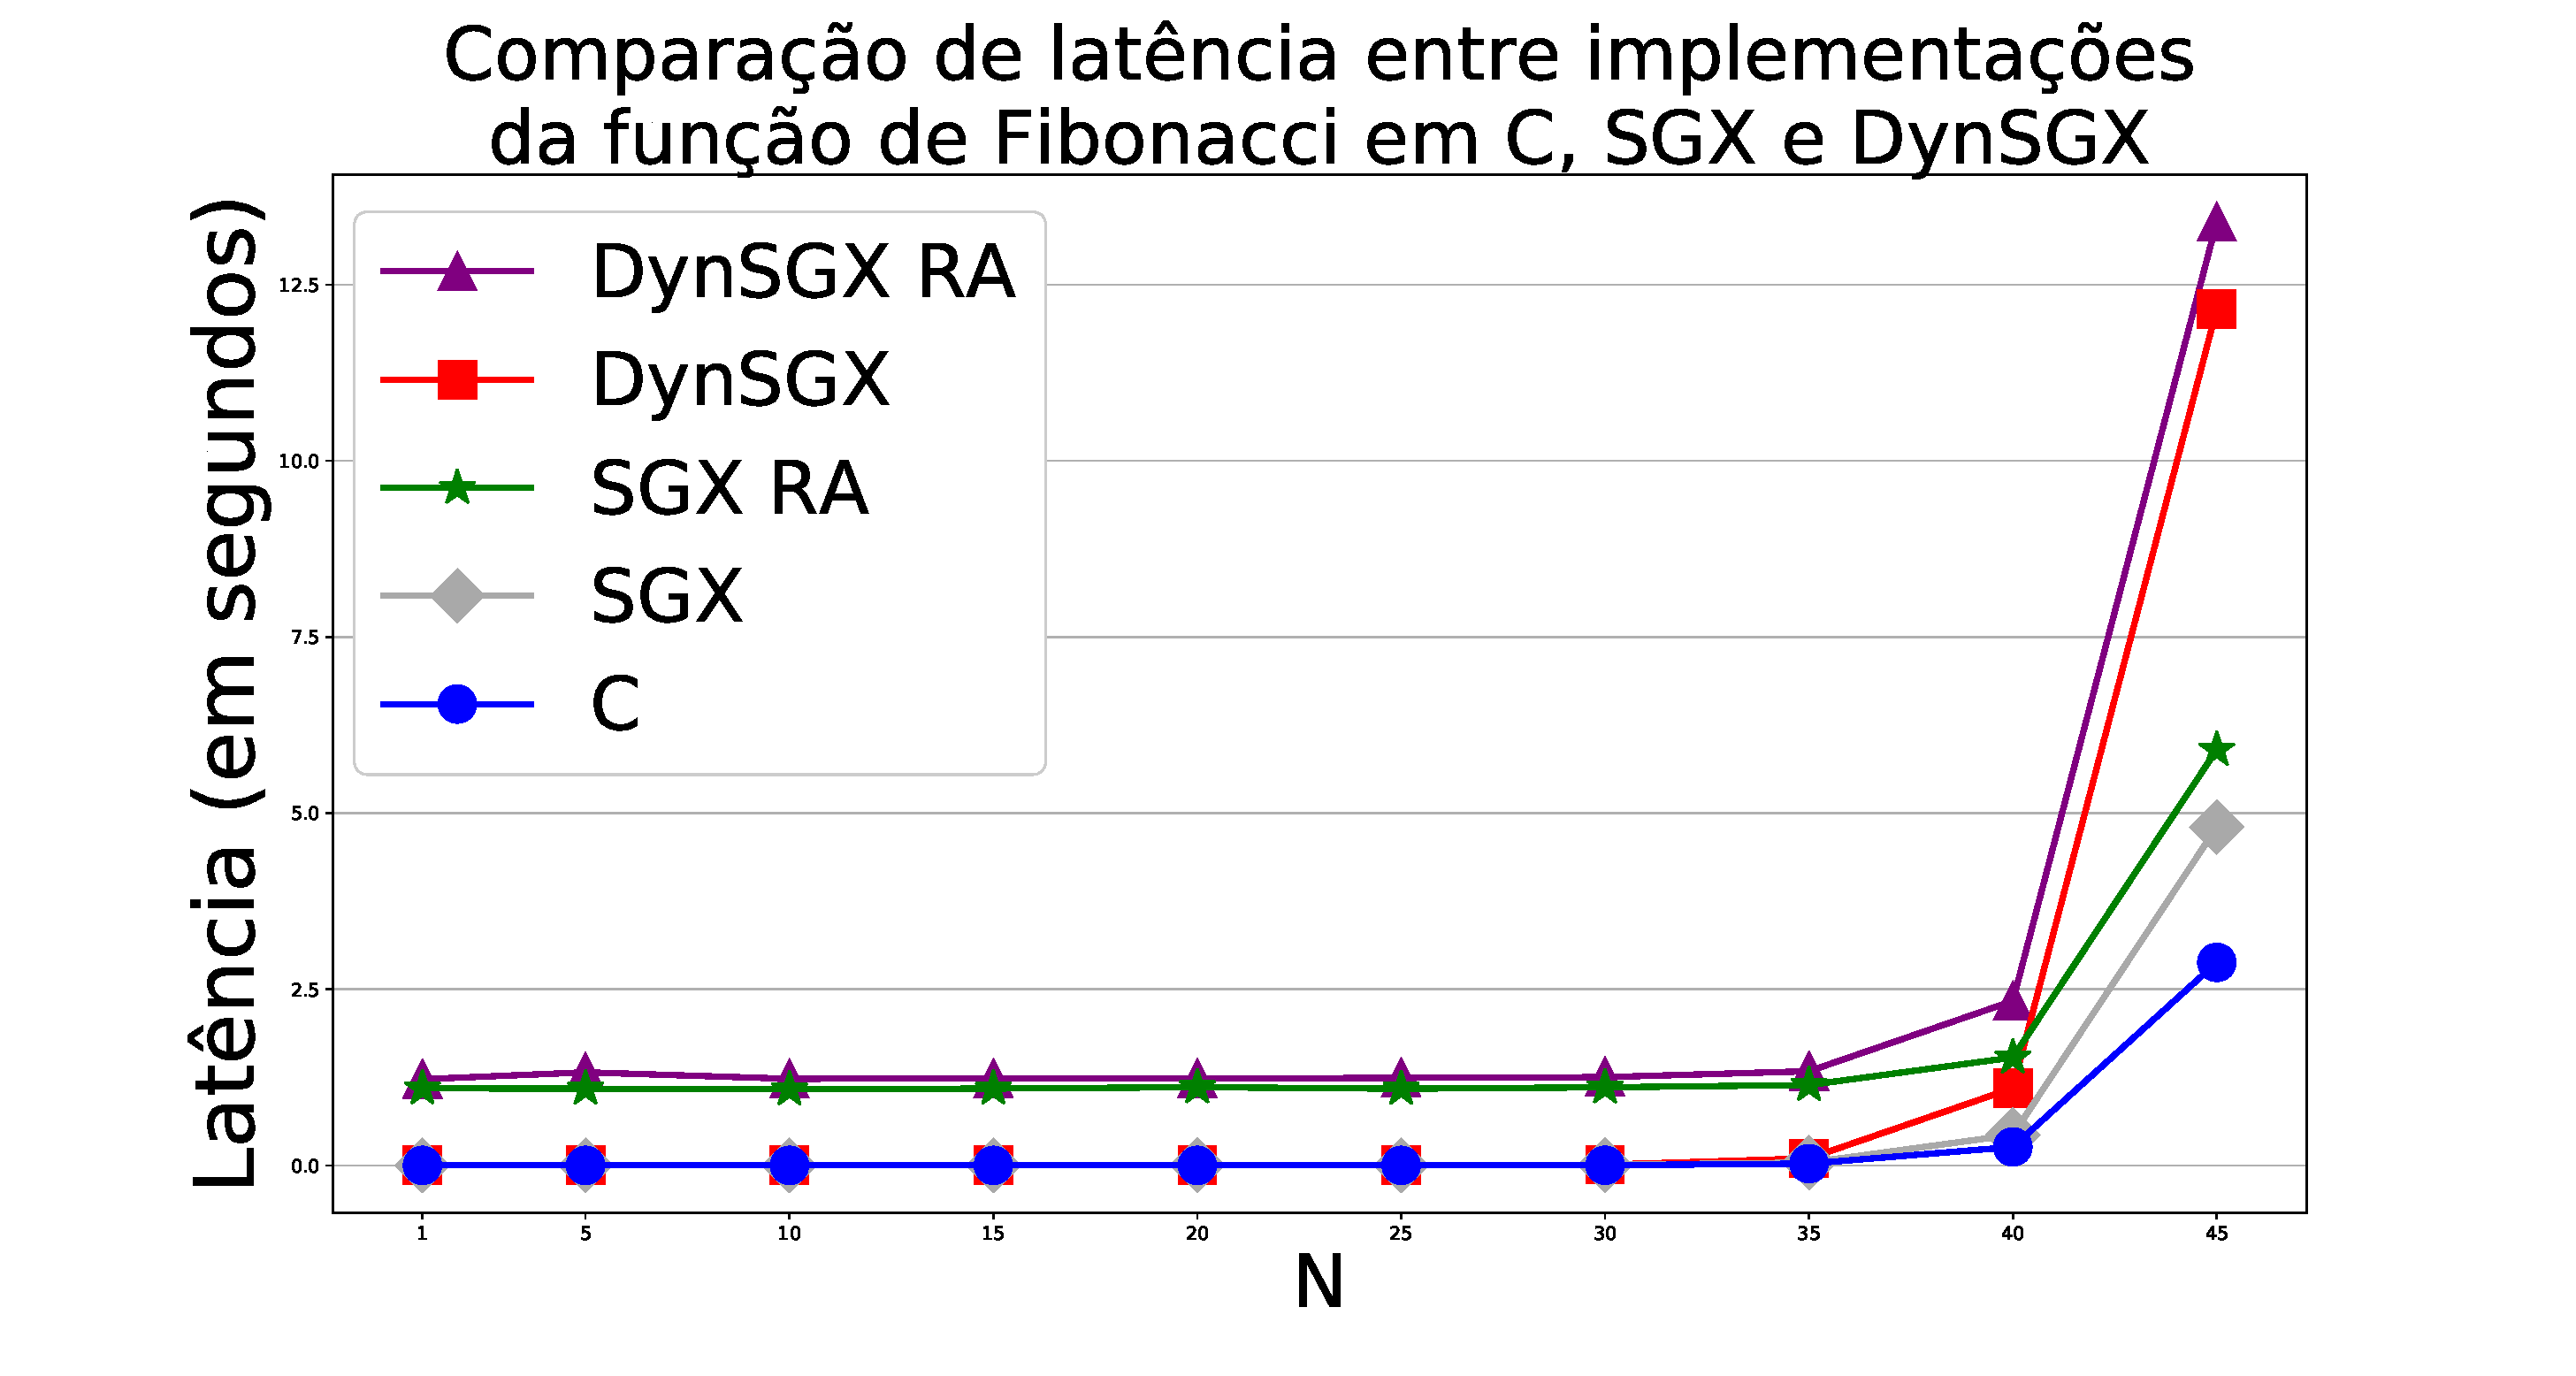
\includegraphics[width=5in]{img/fib_results}
    \label{fig:fib_results}}
    \caption{Comparação de latência entre as implementações em C puro, Intel
    SGX, e DynSGX}
    \label{fig:exp_results}
\end{figure*}

Os experimentos foram constituídos de duas partes. A primeira parte buscava
comparar a latência para computar a função \textit{sum\_array} para \textit
{arrays} com tamanhos de $2$, $4$, $8$, $16$, $32$, $64$, $128$, e $256\ MB$.
A Figura~\ref{fig:sum_results} mostra a mediana dos valores de latência obtidos
nesta parte do experimento. Este experimento serve para nos mostrar o
comportamento do uso de DynSGX com funções iterativas, especialmente quando há
um consumo de memória que extrapola a memória disponível na EPC.

A segunda parte do experimento visa comparar a latência para computar a função
\textit{recursive\_fibonacci} assumindo os valores de $1$, $5$, $10$, $15$,
$20$, $25$, $30$, $35$, $40$, e $45$ para a variável $n$. A Figura~\ref
{fig:fib_results} mostra a mediana dos valores de latência obtidos nesta parte
do experimento. Este experimento é importante para mostrar o comportamento do
uso de DynSGX com funções recursivas.

Em ambas as partes do experimento, para cada tamanho de \textit{array} e para
cada valor da variável $n$, 30 repetições foram executadas. Os resultados
obtidos nestes experimentos têm distribuição enviesada. Por este motivo,
escolhemos a mediana como medida de tendência central utilizada na análise feita.

\subsection{Discussão}
\label{subsec:dynsgx_avaliacao_discussao}

Como pode ser visto na Figura~\ref{fig:exp_results}, ambas as implementações que
usam SGX e DynSGX sempre geram uma sobrecarga considerável se comparadas a
implementação em C puro, que não se preocupa com segurança e privacidade de
dados do usuário. Esta sobrecarga acontece por dois motivos principais: ($i$) o
tempo necessário para realizar o processo de atestação remota, e ($ii$) a
necessidade de cifrar e decifrar dados constantemente.

A partir dos resultados obtidos nos experimentos, pode-se observar também que
para processar funções iterativas, DynSGX apresenta apenas uma pequena
sobrecarga, de aproximadamente $2,5\%$, comparando-se com o uso de SGX.
Este comportamento pode ser observado em ambos os casos quando é necessário
realizar o processo de atestação remota, e quando o canal de comunicação seguro
já foi estabelecido. Neste cenário, nós consideramos os benefícios de usar
DynSGX significantes, por adicionar privacidade do código executado no enclave,
e a possibilidade de gerenciar a memória ocupada por código.

Entretanto, é importante observar que o DynSGX pode não ter uma performance
muito boa no caso de funções recursivas. A Figura~\ref{fig:fib_results} mostra
este cenário, onde o tempo de execução da função \textit{recursive\_fibonacci}
cresce exponencialmente à medida que o número de chamadas recursivas cresce.
Neste cenário, DynSGX tem uma performance muito inferior à performance do SGX.
Este comportamento acontece porque com o DynSGX o código das funções reside na
\textit{heap}, que é um segmento de dados, e compete com outras áreas de dados,
como os quadros de dados das chamadas recursivas, por espaço na \textit{cache} 
do processador. Processadores modernos têm \textit{caches} distintas para código
e dados. Deste modo, a implementação SGX tem melhor performance neste cenário
por manter o código da função na \textit{cache} de instruções.
Este comportamento não é limitado ao DynSGX. Uma implementação C pura ou SGX de
um algoritmo recursivo que armazene código na \textit{heap} também obterá alguma
sobrecarga.

Em relação aos aspectos de segurança mencionados na Seção~\ref
{sec:dynsgx_vulnerabilidades}, é importante evidenciar que desabilitar os
canários de pilha e habilitar a execução da \textit{heap} não necessariamente
implicam riscos para o dono do \textit{hardware} executando o \texttt{DynSGX
enclave}, uma vez que em ambientes de computação na nuvem é possível configurar
outras camadas de segurança. Por exemplo, o \texttt{DynSGX enclave} poderia ser
executado em um ambiente isolado como uma máquina virtual.

Por fim, na Tabela~\ref{tab:dynsgx_sgx_comparison} é apresentada uma comparação
das vantagens e desvantagens de cada uma das três implementações consideradas
nos experimentos.

\begin{center}
    \begin{table}
        \caption{Comparação de performance entre as implementações em C puro,
        SGX e DynSGX}
        \label{tab:dynsgx_sgx_comparison}
        \centering
        \begin{tabular}{|c|c|c|c|c|c|c|}
            \cline{2-7}
            \multicolumn{1}{ c |}{} & \multicolumn{2}{ c |}{\textbf{Segurança}} & \multicolumn{2}{ c| }{\textbf{Privacidade}} & \multicolumn{2}{ c |}{\textbf{Performance}} \\ \cline{1-7}
            \textbf{Impl.} & \textbf{dados} & \textbf{código} & \textbf{dados} & \textbf{código} & \textbf{iterativo} & \textbf{recursivo} \\ \hline
            C puro &  &  &  &  & Alta & Alta \\ \hline
            SGX & \ding{51} & \ding{51} & \ding{51} &  & Média & Média \\ \hline
            DynSGX & \ding{51} & \ding{51} & \ding{51} & \ding{51} & Média & Baixa \\ \hline
        \end{tabular}
    \end{table}
\end{center}

\section{Considerações}
\label{sec:dynsgx_consideracoes}

As limitações existentes na tecnologia Intel SGX levou à construção da
ferramenta DynSGX, apresentada neste capítulo. A ferramenta proposta facilita o
desenvolvimento de aplicações que fazem uso de SGX, uma vez que não requer que o
desenvolvedor adquira conhecimento sobre as APIs da tecnologia. A ferramenta
também possibilita a gerência de memória ocupada pelo código de uma aplicação, o
que não era possível no modelo de programação convencional do SGX.

Considerando a avaliação conduzida sobre a ferramenta, foi mostrado que a
ferramenta possibilita obter privacidade também do código da aplicação a ser
executada dentro do enclave, gerando apenas uma pequena sobrecarga em relação a
aplicações SGX comuns em alguns casos.

Por fim, é necessário ressaltar que DynSGX não deve ser aplicado em todos os
cenários. Um dos cenários que se mostrou impróprio para o uso de DynSGX é o das
funções recursivas que possuem uma quantidade exponencial de chamadas recursivas.
Neste caso, o desenvolvedor deve analisar se o custo decorrente do uso do DynSGX
é justificado pelos ganhos de privacidade do código e gerenciamento de memória
consumida por código.